%%%%%%%%%%%%%%%%%%%%%%
\documentclass{singlecol-new}
%%%%%%%%%%%%%%%%%%%%%%

\usepackage{natbib,stfloats}
\usepackage{mathrsfs}
\usepackage{listings}           
\usepackage{graphicx}
\usepackage{multirow}
\usepackage[table,xcdraw]{xcolor}

\def\newblock{\hskip .11em plus .33em minus .07em}

\theoremstyle{TH}{
\newtheorem{lemma}{Lemma}
\newtheorem{theorem}[lemma]{Theorem}
\newtheorem{corrolary}[lemma]{Corrolary}
\newtheorem{conjecture}[lemma]{Conjecture}
\newtheorem{proposition}[lemma]{Proposition}
\newtheorem{claim}[lemma]{Claim}
\newtheorem{stheorem}[lemma]{Wrong Theorem}
\newtheorem{algorithm}{Algorithm}
}

\theoremstyle{THrm}{
\newtheorem{definition}{Definition}[section]
\newtheorem{question}{Question}[section]
\newtheorem{remark}{Remark}
\newtheorem{scheme}{Scheme}
}

\theoremstyle{THhit}{
\newtheorem{case}{Case}[section]
}

\makeatletter
\def\theequation{\arabic{equation}}

%\JOURNALNAME{\TEN{\it Int. J. System Control and Information
%Processing,
%Vol. \theVOL, No. \theISSUE, \thePUBYEAR\hfill\thepage}}%
%
%\def\BottomCatch{%
%\vskip -10pt
%\thispagestyle{empty}%
%\begin{table}[b]%
%\NINE\begin{tabular*}{\textwidth}{@{\extracolsep{\fill}}lcr@{}}%
%\\[-12pt]
%Copyright \copyright\ 2012 Inderscience Enterprises Ltd. & &%
%\end{tabular*}%
%\vskip -30pt%
%%%\vskip -35pt%
%\end{table}%
%}
\makeatother

%%%%%%%%%%%%%%%%%
\begin{document}%
%%%%%%%%%%%%%%%%%

\setcounter{page}{1}

\LRH{J. Dantas et~al.}

\RRH{SERIN - Semantic RESTful Interfaces}

\VOL{x}

\ISSUE{x}

\PUBYEAR{2017}

\BottomCatch

\CLline

\subtitle{}

\title{SERIN - Semantic RESTful Interfaces}

%
\authorA{Jose Renato Villela Dantas}
%
\affA{PPGIA,\\ Universidade de Fortaleza,\\ Fortaleza, CE, Brazil \\
Fax: +55 85 34773061 \qquad E-mail: jrdantas@edu.unifor.br}
%
%
\authorB{Pedro Porfirio Muniz Fariaz}
\affB{PPGIA,\\ Universidade de Fortaleza,\\ Fortaleza, CE, Brazil \\
Fax: +55 85 34773061 \qquad E-mail: porfirio@unifor.br}
%

%
%\authorA{Fusheng Wang\footnote{Work done while working at Siemens Corporate Research.} }
%
%\affA{Department of Biomedical Informatics, Emory University
%\newline
%36 Eagle Row, Ste 589, Atlanta, GA 30322, USA}
%
%
%
%\authorB{\footnotesize Cristobal Vergara-Niedermayr\footnote{Work done while working at Siemens Corporate Research.}}
%\affB{Oracle \newline
 %New Jersey, USA}
%
%
%\authorC{Peiya Liu}
%\affC{Department of Integrated Data Systems, Siemens Corporate
%Research \newline 755 College Road East, Princeton 08540, USA}

\begin{abstract}
This chapter presents the semantic interfaces proposal. It defines the SERIN specification and its address convention.
This chapter compares the presented SERIN specification with similar approaches. Several examples were provided that implements the web services in the description languages described in chapter \ref{chapter:swsdescription} and we compare them to a similar implementation in SERIN.
\end{abstract}

\KEYWORD{SERIN; restful web service; semantic web service; semantic interface.}

\REF{to this paper should be made as follows: Dantas, J.R.V. and Farias, P.P.M. (2017) `SERIN - Semantic RESTful Interfaces', {\it International Journal of Web and Grid Services}, Vol. x, No. x, pp.xxx\textendash xxx.}

\begin{bio}
	Jos\'{e} Renato Villela Dantas graduated as Tecnólogo em Processamento de Dados from Universidade Presbiteriana Mackenzie (1998). He is currently project manager at Serpro. Has experience in Computer Science, focusing on Database, acting on the following subjects: ontology, conceptual navigation, semantic web and open hypertext.\vs{9}
	
	\noindent Pedro Porf\'{i}rio Muniz Farias has bachelor at Bacharelado em Ciencias da Computacao from Universidade Estadual do Ceará (1988), master's at Computer Science from Instituto Militar de Engenharia (1991) and doctorate at Computer Science from Universidade Federal do Rio de Janeiro (1998). Has experience in Computer Science, acting on the following subjects: internet, ontologias, engenharia de software, xml and function points.
\end{bio}


\maketitle

\section{Introduction} 
\label{sec:introduction}

\section{Related work} 
\label{sec:relatedwork}

\subsection{hRESTs with MicroWSMO}
\label{sec:hrests}

\subsection{RESTdesc}
\label{sec:restdesc}

\subsection{ReLL}
\label{sec:rell}

%%%\subsection{Swaggle}
%%%\label{sec:swaggle}
%%%
%%%\subsection{Express}
%%%\label{sec:express}
%%%
%%%\subsection{RESTfulgrounding}
%%%\label{sec:restfulgrounding}
%%%
\section{Semantic RESTful Interface}
\label{sec:serin}

\subsection{Theoretical background}
\label{sec:serin-theory}

\subsubsection{The SERIN scenario} 
\label{sec:serinscenario}
We are supposing that the web consists of a set of hosts. A subset of these hosts can agree 
in provide resources following the same abstract interface, i. e., the resources are instances of the same classes and are accessible with a similar set of web services.

Some examples: a set of book stores B1, B2, and B3, can agree in offer resources of the class \textit{Book}. 
In spite of the resource are instances of the same class, the books offered by the bookstore B1 are different from the books offered by the bookstore B2. 
The bookstore B3 also offers different books from the bookstore B1 and B2. 
A set of travel agencies can agree in offer resources of the class \textit{Travel}. 
A set of banks can agree in offer resource of the class \textit{Account}. 
A set of sensors in the Internet of Things (IoT) can offer resources of the class \textit{Temperature}. 
The temperature measured by the sensor S1 is different from the temperature measured by the sensor S2. 

Behind this supposition, 
\begin{itemize}
	\item We split the knowledge in two levels: the shared knowledge and the particular knowledge. We consider a scenario where a client is looking for particular information from several hosts. This search requires a formalization of a shared knowledge that enables the communication and a particular knowledge that is the information that the host knows and the client desires but it does not know.
	\item The resources has a granularity analogous to the granularity of a record of a database or the granularity of an object in the object oriented paradigm. The resources follow a set of integrity constraints. Mechanisms for integrity checking are important for data based applications. This work consider the web as a huge distributed database where each host provides its own data. These data can be combined to compose a major information.     
	\item Each host has a local closed word assumption with respect of the set of resources that it provides. The definition of integrity constraint mechanisms in this work intends to approach the restrictions presented on the closed world assumption, that exists on relational databases, to the open world assumption that is adopted by the semantic web technologies.
	\item If different hosts provide resources that follow the same interface, these resources are accessible using a similar set of Restful web services whose URL follow a pattern of formation. This work establishes an address convention for the URLs used to request the web services. This address convention contributes to the web service discovery process because it is previous known by the clients that searches for web services. 
\end{itemize}

This scenario is different from the traditional semantic web scenarios because:
\begin{enumerate}
	\item In general, the semantic web models the shared knowledge. Semantic web main goal is the adoption of technologies that enables machines to understand the read information. 
	Semantic web specifies the use of ontologies and data exposed in RDF format. 
	The ontologies usually publish data as instances in an ontology. 
	All these information is considered a shared knowledge. The ontology definition is omitted about the particular knowledge.
	In our scenario, the data existing in a host is not considered a shared information. In spite of being represented in RDF format, it is not contained inside an ontology. A host provides a RDF representation in response for a client's request.
	\item The semantic web does not refer models to the content of messages. 
	% a ontologia se refere a conhecimento compartilhado. entretanto as mensagens servem para que voce solicite ou informe a cerca do conhecimento nao compartilhado. Isto eh, quando A pergunta algo que somente B sabe responder.
	\item The granularity  of semantic web are RDF triples. The most common media type for data in the semantic web is the RDF. RDF is basically a triple in the format \textit{subject-predicate-object}. 
	This granularity is lower than the one necessary to represent a more complex object like a record in a relational database. 	
	The representation of a relational database record in RDF needs a set of triples.  
	Even if we consider a set of RDF triples as the representation for a complex object, this is an informal definition since there is no mechanisms in the RDF specification to formally describe the relation between the triples.
	
	On the Web, RDF data are distributed, partial, and incomplete. 
	A piece of information can be provided by the composition of data provided by several hosts distributed on the Web. These data can be part of a composed data.
	Each part can have a RDF schema that represents the metadata definition for this partial data.
	Furthermore this data is considered incomplete because there is no metadata schema that formally describes the whole data and there is no formalism that guarantee that a new piece of data can be found in an unknown server. 
	
	Our proposal defines \textit{RDF instances} as an extension to RDF triples. The \textit{RDF instances} intend to provide a mechanism to define a granularity that is a set of triples. This mechanism is sufficient to represent complex objects like database records.    
	%TODO (ver) explicar a analogia entre sparql e os servicos serin
	\item The queries normally are written in SPARQL. Hosts in the semantic web usually provide SPARQL endpoints as consultation mechanisms to their particular data. The use of such endpoints requires from the client a knowledge about the SPARQL language and the host metadata model. Our approach proposes a consulting mechanism based on web services following an address convention. The requests to these web services can substitute the SPARQL queries in most of the times. 
	%TODO (ver) comentar com Porfirio sobre a existencia de alguns sites com web apis que fornecem um endereco para acesso.
	\item The semantic web is mainly a set of repositories that are updated only by their respective owners because no integrity restrictions is modeled. Semantic web is essentially a read-only environment where each host is responsible to maintain its own data. Nowadays there is still little effort in provide mechanisms for a read and write Web.
	The information sent in a response does not have an associated schema to describe the data. 
	Despite ontology concepts can describe parts of the data, the existence of a full data schema provides a minimal set of rules for integrity verification.
	
	We consider a scenario where a client intends to send requests to update data in an external host database after an initial read query. This intention can be noticed in scenarios like e-commerce, e-government, and the first example for web semantic where a automatic agent intends to schedule an appointment. 
	The persistence of data requires mechanisms to verify the data integrity in order to guarantee the consistence of data in the host database.  
	\item The open world assumption (OWA). This assumption is useful in scenarios, like the semantic web, where the knowledge base is considered incomplete, i.e., it is assumed that not all facts and axioms that make up the application domain are known.
	Our approach adopts the local \textit{closed world assumption} (LCWA). This assumption enables a set of mechanisms for integrity constraints which is necessary in a scenario where clients need to persist data in external hosts.
\end{enumerate}

This scenario is different from the usual semantic web service scenarios because:
\begin{enumerate}
	\item It specifies an abstract interface. The usual web service description languages describe one web service in a host. This is mainly truth for SOAP/WSDL based web services which uses WSDL as description language, sometimes with some semantic enhancement. Some languages can also describe RESTful web services but their are not widely adopted.  
	Despite these description languages are useful for the interaction between a client and the web service, they restrict the discovery of unknown web services since their specifications are not the same.
	Our proposal specifies an abstract interface that describes a category of web services in different hosts that follow the same interface.
	\item Services with the same semantics has URLs with the same pattern. In the Web specification, it is not possible to determine the type of a resource by inspecting a URL. A pattern is useful because it eases the identification of the resource that a URL represents.  
	\item There is no matching between a user requirement and the web service description. Most of web service discovery process consider some matching process to discover the web service that best attends a given requirement. For several reasons, this matching is always inaccurate.
	
	In this proposal, considering that the abstract interface is known, the clients previously know which service attends their needs. Our proposal intends to avoid the uncertainty of the matching process. In this case, the client always executes a full match when it performs a request. 
	\item An annotated ontology establishes the semantics of the web services. In the semantic web, the usual approaches specifies their own description languages to semantically describe the web services. The most common approaches define an upper ontology with concepts to describe the operations, parameters, and other elements of the web service. In such approaches, the upper ontology is combined to a domain ontology to describe the resources of a web service.
	Our approach proposes the annotations to be inserted in the domain ontology. We consider that only the annotated domain ontology is necessary to describe the web service. 
\end{enumerate}

In the following sections, we first detail the assumptions in the proposed scenario. These assumptions forms the basis for the SERIN specification presented in the latter sections in this chapter. 

\subsubsection{Shared knowledge and particular knowledge}
\label{sec:sharedknowl}
The \textbf{shared knowledge} is the piece of information that the sender and the receptor in a  communication must know to enable both sides to understand the message. 
This knowledge defines that a concept has the same meaning.

Formally, we define \textit{meaning} as a function $\delta(URI) -> C$ that is a mapping from a set of URIs, i.e. the domain set, to a set of concepts, i.e. the image set (Figure \ref{fig:functionmeaning}). 
These concepts represents objects from the real world. The image set can have four types of concepts: a class, i.e. a category of objects; a attribute, i.e. a property that an object has; a relationship, i.e. the relation between two other concepts in the set; and an instance, i.e. the individual that is the type of a class. 
Each concept has an URI that uniquely identifies it.

\begin{figure}[!b]
	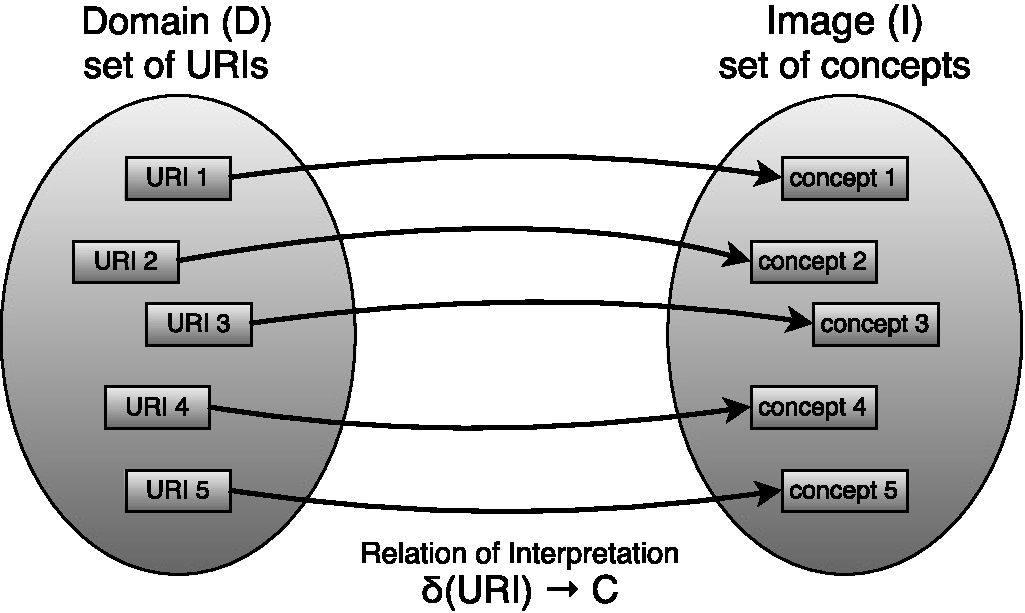
\includegraphics[scale=.6]{images/conjunto-interpretacao-compartilhada.pdf}
	\centering
	\caption{The function $\delta(URI) -> C$ maps a URI in the domain set to a concept in the image set.}
	\label{fig:functionmeaning}
\end{figure}

The \textit{meaning} of a concept is shared between a sender and a receptor in a communication when this concept has an URI in the sender that is associated to the same concept for a URI in the receptor. Both sender URI and receptor URI are associated to the same concept from the real world.
This association indicates that sender and receptor has a \textit{shared understand} about the concept \textit{meaning}. 

On the Semantic Web, an ontology is used to represent the shared knowledge. 
An ontology is a document that implements the function $\delta(URI)$, i.e. it maps URIs to concepts.
This mapping provides the semantics for the URIs. 
Any machine that access such document is aware about the concepts defined in the ontology, i.e. the machine knows the URI that represents each concept. 

For example, a book ontology (Figure \ref{fig:bookontology}) presents concepts, like \textit{Book} and \textit{Author}, and relationships, like \textit{Book has Author}. These concepts are known by a host in a bookstore, which provides information about its books, and by the client who wants to know these information.  
A client can send a request to a host asking for Book information. The client receives the desirable response because him and the host agree about the Book concept. 

\begin{figure}[!htb]
	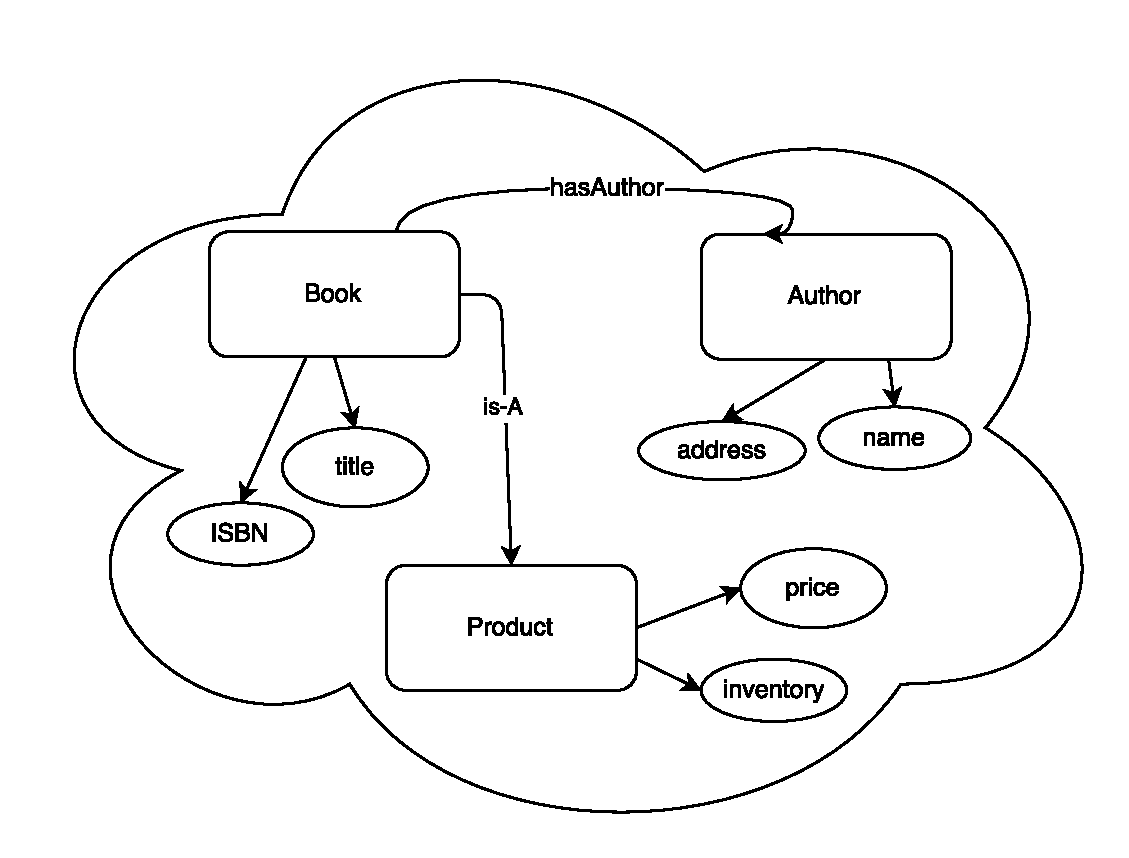
\includegraphics[scale=.55]{images/book-ontology.pdf}
	\centering
	\caption{Book ontology: a shared knowledge.}
	\label{fig:bookontology}
\end{figure} 

The existence of a shared information assumes there is also some information that is not shared. Indeed, the hosts on the Web can provide a complementary information that is exclusively stored in their particular databases. 
We call this information as \textbf{particular knowledge}. 
This is the information that the client doesn't have and the one he is looking for. 
The particular knowledge is complementary to the shared knowledge.

The formalism for the particular knowledge follows the same formalism for the shared knowledge but there is a slight difference. The particular knowledge is a mapping $\delta(URI) -> C$ that is exclusive for one host. It means that, given a concept $C_i$, only a host A maintains the mapping $\delta(URI_A) -> C_i$. A second host B can maintain the mapping $\delta(URI_B) -> C_i$. Host A is not aware about the object represented by $URI_B$ while the host B is not aware about the $URI_A$.

\begin{figure}[!htb]
	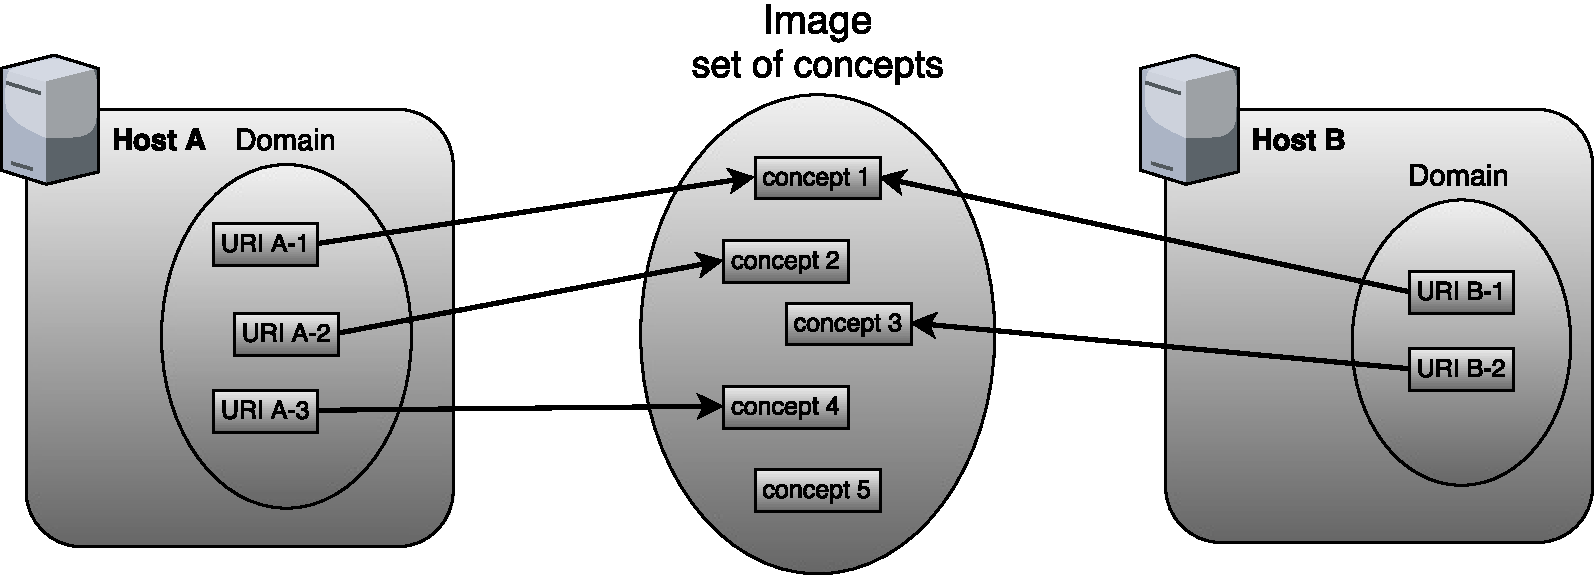
\includegraphics[scale=.45]{images/conjunto-interpretacao-particular.pdf}
	\centering
	\caption{In a particular knowledge representation, each host has some exclusive relations $\delta(URI) -> C$.}
	\label{fig:particularknowledge}
\end{figure} 

In the example of the Bookstore (Figure \ref{fig:bookprivateknowledge}), a web service can provide particular data about a book. The same request sent to two different hosts returns two different responses to the client. The concepts in the output message are the same but their values are different. The highlighted data, price and inventory, are exclusive to each host. 

\begin{figure}[!b]
	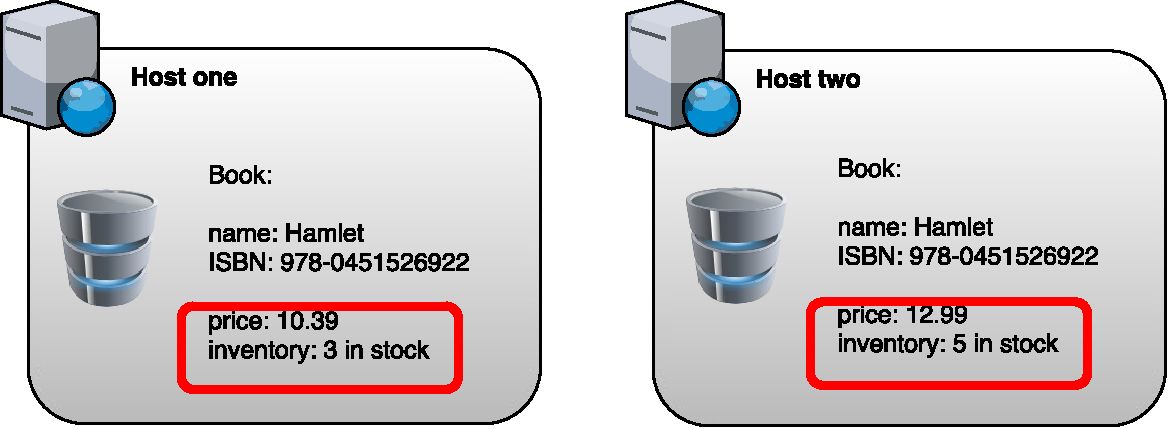
\includegraphics[scale=.6]{images/Book-private-knowlege.pdf}
	\centering
	\caption{Example of private knowledge.}
	\label{fig:bookprivateknowledge}
\end{figure}

The distinction between the shared and the particular information in the Book Selling scenario evidences the advantages of semantic abstract interfaces.
The main advantage is that the semantic abstract interface enables the clients to obtain data that only one host maintains because both client and host are aware about the data schema. 
A second advantage is that is possible to establish comparison among data from different hosts because their metadata are described by the same interface.
%The main difference between particular and shared knowledge resides on the data content that they own. 

A consultation for the shared information about a book always returns the same title and the same author. It doesn't matter which host answer the request. The client always gets the same data values given the same book id. 

In contrast, a request for a particular information returns an information that is specific for each host. 
Host A has values of price and inventory that are different from Host B. 

Observe that the client must know the same concepts to reach the values that only the host owns. 

\subsubsection{Local closed world assumption}
A scenario where it is possible to observe the advantages of semantic abstract interfaces is the data maintenance on the Web. 
This scenario consider a database, hosted in a server on the Internet, where a client agent can send information for persistence. 
The client agent must obey the database schema otherwise it risks to send inconsistent data. 

In this scenario, the semantic abstract interfaces can work as a database schema. It is possible to establish a mapping between classes and properties in the ontology with tables and fields in a relational database.

Read and write operations at data centric applications usually considers one of two assumptions: the open world assumption (OWA) or the closed world assumption (CWA).

Open World Assumption considers that an information is not false but unknown if it is absent in a database or it cannot be logically inferred from a known information. OWA is well applied in the context of World Wide Web. This environment provides no guarantee that an agent can always obtain complete or consistent information about a fact. 

On the other hand, the Closed World Assumption that only the information that exists in the database, or that can be proved from available data, is true. All other information is considered false. Many application domains consider the closed world assumption appropriate because it explicit describe only the positive facts leaving the truth of the negative facts as a default. This is called the \textit{negation as failure} principle \citep{clark1978negation}. CWA applies to systems that have complete information as it is in the relational database.

Although OWA is a proper model to the Internet, it is sometimes desirable to adopt CWA capabilities. 
It is preferable, for example, when data is retrieved from a relational database, or the data can somehow be considered complete in respect to the domain question.

In this situation, it is necessary to define a model that follow OWA but considers some CWA characteristics. The Local Closed World Assumption (LCWA) \citep{Sengupta2011} combines the OWA with the CWA in a model that extends capabilities from closed world, of completeness and integrity verification, to knowledge representation languages on the open world. 

\subsubsection{The role of interfaces}
Basically the interfaces contributes for the partition of a system into multiple computational layers, which can be, for example, a program internal layer, or distributed computing APIs (Application Programming Interfaces). 

Generally an interface is a contract that defines which data a service requester and a service provider can exchange, and how this exchange occurs, i.e., which methods are allowed to perform over the data. Any service provider that agree with this contract must implement the web services according to the interface specification.

The adoption of interfaces as a mechanism for abstraction is widely disseminate in the computer science. 
A software interface may refer to a wide range of different types of interface at different ``levels'': an operating system may interact with the computer hardware; applications or programs running on the operating system may need to interact via system calls; and in object oriented programs, objects within an application may need to interact via methods.

In object-oriented languages like, for example, Java and C++, the term interface is often used to define an abstract type that contains no code, and usually no data, but defines behaviors as method signatures. 
Interfaces are composed by attributes and abstract methods.
A class implements an interface when it implements code and data for all the abstract methods corresponding to that interface. 
The object-oriented paradigm promotes the reuse of existing interfaces, i.e., a software agent can easily use shared interfaces in order to follow the contract that the interface defines.

%TODO (ver) se inclui essa discussão sobre interoperabilidade: 
%Interfaces are widely used to facilitate the interoperability between systems.
%inicialmente, a interoperabilidade ocorria através da troca de arquivos. 
%The CORBA IDL (interface definition language)... a interoperabilidade ganha força com a proposição do CORBA.
%Interfaces no CORBA tinham dependencia de localizacao. perguntava pro ORB e ele dizia onde estava o serviço. tinha a vantagem de não saber onde estava. 
%"nao me lembro como age quando a interface tem varios metodos em varios servidores." 

The concept \textbf{abstract interface} reinforces the idea of an interface that several web service providers can implement at the same time. The abstract interface is not bounded to any particular service. 
There is a subtle distinction between the usual web service descriptions and the abstract interfaces. 

When they are applied to the Web environment, the web services adopt interfaces to provide a syntactic description of the available operations in a host.  
The WSDL 2.0 specification defines a set of interfaces as one of its components. WSDL 2.0 also specifies a set of binding components as part of the web service description. In this language, the interface is an integral part of the concrete web service implementation.
We don't consider the WSDL 2.0 interface as an \textbf{abstract interface} because it is tightly coupled to its implementation. 

In contrast, the abstract interfaces are decoupled from the web services that they describe. 
The same abstract interface can describe not only one specific service in a host but a category of web services that has the same inputs, outputs, and it performs the same operation.
It is not the host that provides the web service that specifies the abstract interface. 
This host follows a web service specification defined and shared elsewhere on the Web. 

%TODO (ver) se faz uma seção para explicar os elementos que compoem a sintatica da interface
%explicar que existem entradas, saidas e nome (assinatura). Depois dizer como formar a semantica desses elementos.

\subsubsection{The definition of Resource}
\label{sec:resourcedefinition}
The definition of a resource on the web and in the REST architecture is embracing. Anything in these environments can be a resource. This section presents the definition of resource that is adopted in this work.

W3C specification of the Web Architecture doesn't limit the scope of what might be a resource. 
The term \textit{resource} is used for whatever might be identified by an URI.
It is conventional on the Web to identify Web pages, images, product catalogs, etc. as \textit{resources}.
The Web architecture \citep{webarch} defines the term \textit{information resource} as the set of characteristics that can be conveyed in a message. 
This set of characteristics distinguish one resource.

For the REST architecture, the resource is the key abstraction of information. 
A \textit{resource} is any information that can be named. 
This includes documents, images, services, non-virtual objects (e.g. a person) and even sets of other resources. 
Any concept that might be targeted of a hypertext reference must fit within the REST definition of a resource.

According to these definitions, a resource can be either a single object and a set of objects. For example, in a bookstore system, a client can make three different requests to get information about books. 

\begin{lstlisting}
Request 1: GET /book/978-8575036709
\end{lstlisting} 

\begin{lstlisting}
Request 2: GET /book/moby_dick
\end{lstlisting} 

\begin{lstlisting}
Request 3: GET /book
\end{lstlisting} 

The first request is more restrictive because it has an input with an identification for one book, the ISBN 978-8575036709. This web service responses with only one resource that represents one book. The second request, with a book title as input, can receive a set of books that have the same title but different editions. The third request is more wide and it responses with a set of resources that represents all books. In this situation, the whole set can also be considered a resource.

SERIN specification defines a new concept called RDF instance \citep{Lira2014a}. 
An RDF instance is a set of RDF triples that represents the instance of a class in the semantic interface. 
All RDF triples share the same subject. 
This way, the subject URI in the component triples identifies an RDF instance. 
However, not all triples with the same subject can be an RDF instance.
SERIN annotation in classes and/or properties in the interface indicate restrictions that are necessary to consider the triples as an RDF instance.

For this work, an RDF instance can be considered a resource.
SERIN web services exposes RDF instances as the resources in a host. An RDF instance is the atomic unity of data in a response for a SERIN web service. 
The host and the client exchange RDF documents that can contain one or more instances. 

\subsubsection{Semantic Interfaces}
\label{sec:semanticinterface}
Interfaces have been successfully used as an abstraction to register a syntactic pattern, whose semantics is previously and informally defined, that systems adopt in order to interchange data. 
The semantics of interfaces is usually informal. It is informed through system documentation, training courses, or personal communication between the stakeholders.

%TODO (ver) se vai pesquisar: 
%como fazer para os web services restful simularem uma operação que executa algo que não seja somente devolver dados. por exemplo, como fazer um método que retorna o tamanho de uma string qualquer informada pelo cliente.
%

The informal definition of semantics and the syntactical elements of the interfaces provide a minimal model  that enable the execution of some task over web services, mainly in the mediation between a web service and a client agent. 
Despite this informal semantics is enough for human comprehension, it is not adequate for software agents. The addiction of semantics to the service descriptions can raise the discovery process to a higher level of machine processing.

This work adopts the concept of \textbf{semantic interface} as an abstract interface whose semantics is expressed using semantic web standards. 
This means that an ontology represents an interface.

The abstract semantic interfaces must be public and shared to anyone that wants to provide resources in hosts and the ones that need to consume these resources.
When a new host wants to implement web services following a previously defined contract, it can reuse the same abstract semantic interface.
The abstract interface inserts semantic description to the service syntactic elements of a web service inside a host. 

The shared aspect is important for information exchange. 
It is assumed that an ontology is a set of concepts: classes, properties, and instances, with meaning that everyone, that wants to adopt the ontology, previously know.
It is also assumed that the semantics of concepts in an ontology has been informally defined and communicated. As primitive terms of a formal system, such primitive concepts can be used to formally define new concepts.

The emphasis about the shared aspect of the knowledge represented by an ontology implies the existence of a non shared knowledge. 
Indeed when an agent A asks the age of an agent B, both must know the concept \textbf{Age}, which is a concept in an ontology that the agents know.
However the value of the agent B age is not in the ontology otherwise agent A already knows the ``age of B'' information. 

In general, an ontology doesn't contain the information that is obtained from the messages that a query requester exchange with a result provider.
Agent A asks to agent B about an information that agent B knows but agent A doesn't know.
This information exchange doesn't modify the shared ontology. 

Thus this work doesn't investigate the mechanisms that develop and maintain the ontology. This work considers that the ontology definition is static, i.e., it is not changed during the web service interaction process.

The ontology doesn't contain the information that is particular to each communication agent. 
However the agents can use it to define how this information is represented.
In a RESTful web service context, the resources inside a host represent the particular information from each agent. 
In other words, resources are instances of an ontology class but they are not contained, neither fully or partially, in the ontology because they are not a previous shared information. 

It should be noted that instances can be contained in an ontology, i.e., they can also be objects inside an ontology. 
In this situation, considering that an ontology is a public and consensual information to any requester agent or provider agent, the instances are also a shared information the same way the classes and properties are.  

For their turn, the particular resources extend the information from an ontology. 
The particular resources can be added to the resources already present in the ontology, i.e. the ontology instances. 
The ontology provides a formal semantics to the particular resources. 
Such particular information associated to the shared information can be represented by RDF instances, according to the following convention:

\begin{itemize}
	\item Each instance is associated to a class and it have the same subject. This subject have an URI that uniquely identifies it. This subject URI identifies the RDF triples that integrates an RDF instance.  
	\item Instances have properties whose domain includes the class that defines the instance. The property domain and ranges are defined in the ontology. The RDF representation that describe resources is
\end{itemize}

For example, in a Bookstore scenario that adopts the Book ontology (see Figure \ref{fig:bookontology} in section \ref{sec:sharedknowl}), information about a Book can be represented as RDF instance as shown in figure \ref{fig:bookrdfinstance}.

\begin{figure}[!ht]
	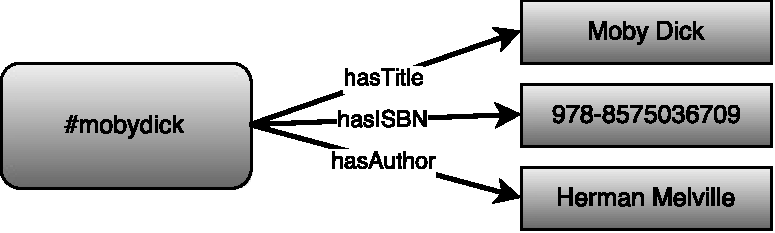
\includegraphics[scale=.7]{images/book-rdf-instance.pdf}
	\centering
	\caption{Example of a Book representation as RDF instance.}
	\label{fig:bookrdfinstance}
\end{figure}

The RDF representation for this RDF instance is:

\begin{lstlisting}[breaklines=true]
<Book rdf:about=#mobydick>
<rdf:type rdf:resource="http://example.com/books.owl#Book"/>
<title rdf:datatype="&xsd;string">Moby Dick</title>
<isbn rdf:datatype="&xsd;string">978-8575036709</isbn>
<price rdf:datatype="&xsd;float">0.99</price>
<books:hasAuthor rdf:resource="http://example.com/books.owl/author#Melville"/>
</Book>
\end{lstlisting}

The ontology concepts can be mapped to web service descriptions, like operations, methods, and other elements in a SOAP/WSDL document or a HTML document that describes a RESTful web service. 
The semantic is usually added to web services through concepts from an ontology associated to the concrete web service description elements.

Therefore this work defines that a software agent implements an ontology when the agent accepts the semantics of the ontology classes, properties, and instances, and the agent also implements the web services that are associated to this ontology.

\subsection{Elements of SERIN}
\label{sec:serin-elements}
Semantic RESTful Interface (SERIN) \citep{Muniz2013a,lira2014semantic} is basically an annotated ontology whose classes and properties characterize uniquely and semantically available resources. 
SERIN specification defines an upper ontology with the annotation properties and a set of additional concepts with their relationships (Figure \ref{fig:serinontology}). 
The annotation properties are divided in two groups: \textit{Operation} and \textit{Integrity Constraint}. 
The additional concepts define the classes \textit{Host} and \textit{Interface} that are necessary for the proposed discovery process.

\begin{figure}[!htb]
	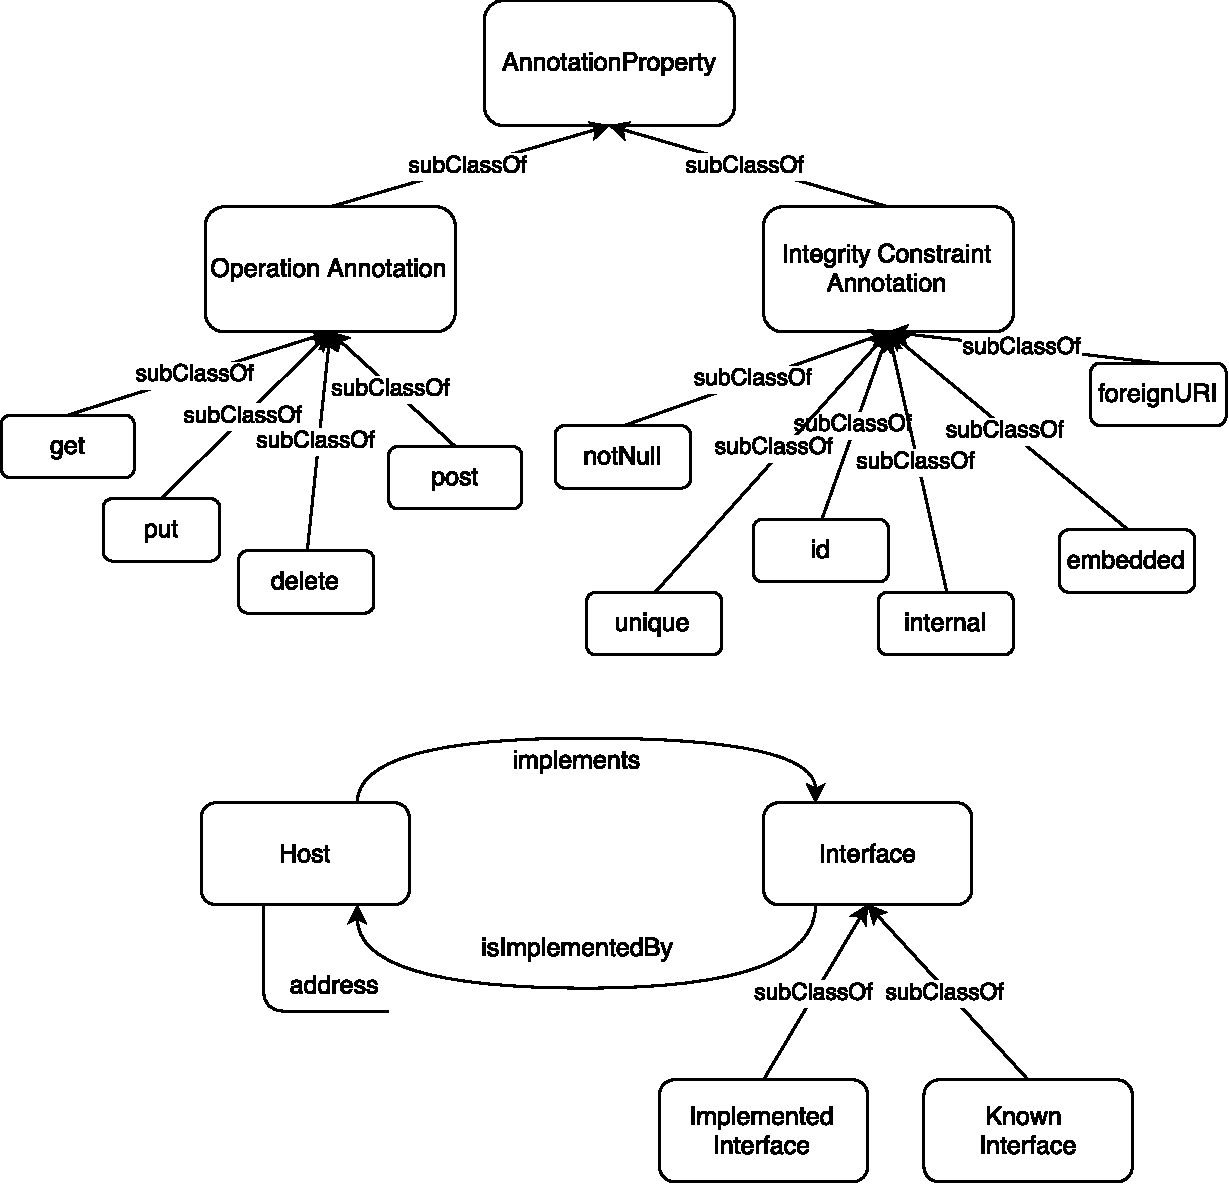
\includegraphics[scale=.5]{images/serin-ontology.pdf}
	\centering
	\caption{SERIN ontology.}
	\label{fig:serinontology}
\end{figure}

%TODO incluir texto sobre implementação
%The annex \ref{anex:serin} shows a full listing of SERIN ontology representation in OWL. SERIN is available on the Internet at \url{http://opendataserin-unifor.rhcloud.com/serin.owl}.

Any domain ontology can import SERIN ontology in order to create a semantic interface. 
The import operation is not mandatory but it contributes to guarantee that the annotations will have the defined conventions. 
It is also useful to identify that domain ontology is a SERIN interface.
An ontology engineer applies the SERIN annotations to the domain ontology classes when he builds an semantic interface.
The resulting annotated ontology is a Semantic RESTful Interface as shown in figure \ref{fig:serinimport}.

\begin{figure}[!htb]
	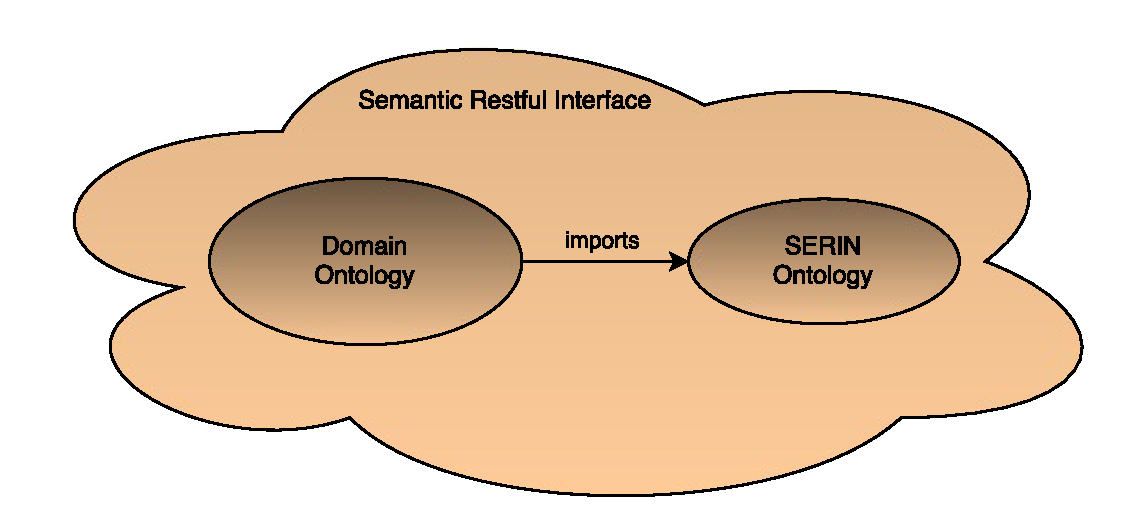
\includegraphics[scale=.55]{images/serin-import.pdf}
	\centering
	\caption{A domain ontology imports the SERIN ontology to create a semantic restful interface.}
	\label{fig:serinimport}
\end{figure}

%TODO (xxx) essas informações estão suscintas e meio soltas, além de já ter falado antes.
%A set of RDF triples, i.e., an RDF instance, represents each resource. An RDF instance has an identifier called \{rdfid\}. The RDF instance granularity is atomic which means that RDF instances can represent a complex object such as a record in a database.

\subsubsection{Operation annotations}
\label{sec:operationannot}
The annotation properties in the group Operation represents the available operations over the services. 
These annotation properties are the SERIN strategy to associate web services to a domain ontology written in OWL. 
Four annotations types can be added to the ontology: \textit{get}, \textit{post}, \textit{delete}, and \textit{put}. 
These annotations indicate the existence of four web service types. 
The four web service types are mapped into the four homonyms relative HTTP methods. 
They define which RESTful Web Service should be implemented for each resource.
In essence SERIN is a domain ontology that receives the described annotations.

%%%\begin{figure}[!htb]
%%%  \includegraphics[scale=.55]{imagens/serin-operation-annotation.pdf}
%%%  \centering
%%%  \caption{The annotation properties representing operations over web services in the SERIN ontology.}
%%%  \label{fig:operationannot}
%%%\end{figure}

The semantics of the four annotations is based in the HTTP methods which are a widely adopted specification on the Web.
Each annotation defines a semantic web service whose URL follow the pattern presented in table \ref{tab:annotations-operation}. 
The identifier \{Host\} represents the URL of a host, viz. a service provider, that implements the semantic interface. The identifier \{interface\} represents the URI that identifies an ontology, viz. a semantic interface.
The identifier \{Class\} represents an annotated class of resources. At least, the identifier \{Property\} represents the annotated property related to a class.

\begin{table}[ht]
	\centering
	\caption{Annotations indicating the web services operations, their location (URL), and their semantics.}
	\label{tab:annotations-operation}
	\begin{tabular}{clp{8cm}}
		\rowcolor[HTML]{C0C0C0} 
		Annotation                                       & \multicolumn{2}{l}{\cellcolor[HTML]{C0C0C0}Description}                                                                                              \\
		\cellcolor[HTML]{CBCEFB}                         & URL       & GET \{host\}/serin/\{Interface\}/\{Class\}/\{rdf:id\}                                                                                    \\
		\rowcolor[HTML]{EFEFEF} 
		\multirow{-2}{*}{\cellcolor[HTML]{CBCEFB}GET}    & Semantics & Receives a resource identifier \{rdf:id\}  as a parameter  and returns its instance                                                      \\
		\cellcolor[HTML]{CBCEFB}                         & URL       & POST \{host\}/serin/\{Interface\}/\{Class\}                                                                                              \\
		\rowcolor[HTML]{EFEFEF} 
		\multirow{-2}{*}{\cellcolor[HTML]{CBCEFB}POST}   & Semantics & Receives a set of RDF triples in the web service body, corresponding to an individual data, and adds it to as an instance of this class. \\
		\cellcolor[HTML]{CBCEFB}                         & URL       & PUT \{host\}/serin/\{Interface\}/\{Class\}/\{rdf:id\}                                                                                    \\
		\rowcolor[HTML]{EFEFEF} 
		\multirow{-2}{*}{\cellcolor[HTML]{CBCEFB}PUT}    & Semantics & Receives an OWL corresponding to the instance identified by \{rdf:id\} and updates the individual data.                                  \\
		\cellcolor[HTML]{CBCEFB}                         & URL       & DELETE \{host\}/serin/\{Interface\}/\{Class\}/\{rdf:id\}                                                                                 \\
		\rowcolor[HTML]{EFEFEF} 
		\multirow{-2}{*}{\cellcolor[HTML]{CBCEFB}DELETE} & Semantics & Receives an instance identifier \{rdf:id\} and removes this individual from the set of instances.                                       
	\end{tabular}
\end{table}

The option to use only four web service types, whose semantics is pre-defined, makes the SERIN semantics much simpler than proposals that specify semantics for SOAP/WSDL web services. 
Semantic Interface properly establishes resources semantics. 
The four possible operation semantics follows CRUD model (create, Read, Update, Delete) usually associated with HTTP verbs.
Since the operation semantics is established, it is only necessary to define the semantics for the properties and return value of the operation.

Each host that implements a semantic interface must implement one RESTful web service for each operation, i.e., for each annotation in a class. 

\subsubsection{Integrity constraint annotations}
\label{sec:constraintsannot}
OWL semantics addresses scenarios where it is not possible to assume a complete knowledge about the data within a domain \citep{tao2010integrity}. 
It is suitable in an environment where data is not complete or, at least, it is reasonable to consider the existence of unknown data, like it occurs on the Internet. 
Two OWL characteristics reinforces these considerations:
\begin{itemize}
	\item The existence of a semantics based on the open world assumption, i.e., the assumption that a formal system can't assume as false but unknown an statement that is not explicit declared or that can't be inferred from any existing axiom.
	\item the absence of the unique name assumption, i.e., two different names can represent the same individual inside a same system. 
\end{itemize}

However in scenarios where services must maintain data that have to be complete, those characteristics difficult the adoption of OWL language to check integrity constraints.
It is though convenient that these services overcome those limitations by implementing mechanisms for integrity constraints.

SERIN implements a set of annotations that enables the validation of integrity constraints based on the local-close world assumption applied to the context of semantic web services that manipulates data.
Such integrity constraints are mechanisms to verify that the requester provides all necessary data to an update operation in a database.  

The fact that it exists a data schema with integrity constraints prevents the requester to send data that cannot be accepted by the server. 
The client agent must obey the constraints when it sends data in an update request, otherwise the server can refuse the request.

Considering an inverse vision from the client agent perspective, the integrity constraints contributes for the client be conscious that it receives a response with consistent data.
For example, if the data schema states that the value in a field must be not null, the client agent can consider that this field will always receive a value. 
The client agent does not need to be aware about receiving partial or incomplete data. 
This enables the construction of a more lightweight program for a client agent because the data schema is previously known. 

%%%\begin{figure}[!htb]
%%%  \includegraphics[scale=.55]{imagens/serin-integrity-annotation.pdf}
%%%  \centering
%%%  \caption{The annotation properties representing the integrity constraints in the SERIN ontology.}
%%%  \label{fig:integrityannot}
%%%\end{figure}

SERIN defines a set of six integrity constraint annotations as detailed in Table \ref{tab:integrityannotations}: \textit{NotNull}, \textit{Unique}, \textit{Id}, \textit{ForeignURI}, \textit{Embedded} e \textit{Internal}. 
In an ontology, all these annotations apply to objects with types \textbf{Datatype Property} or \textbf{Object Property} except for the annotation \textit{Internal} which applies to \textbf{Class} objects
The semantics for these annotations are similar to the semantics for integrity constraints in a relational database model.

\begin{table}[ht]
	\centering
	\caption{SERIN integrity constraint annotations.}
	\label{tab:integrityannotations}
	\begin{tabular}{lp{10cm}}
		\rowcolor[HTML]{C0C0C0} 
		Annotation & Description                                                                                                                                                \\
		NotNull    & A property with a NotNull annotation can 't assume a null value in an relation to an instance.                                                             \\
		\rowcolor[HTML]{EFEFEF} 
		Unique     & It validates that a value for a property is unique inside a host, i.e., the same property doesn't have the same value in two different instance relations. \\
		Id         & It defines the property that is the means to identify an instance in a relation.                                                                           \\
		\rowcolor[HTML]{EFEFEF} 
		ForeignURI & It determines that a property must have a value that is an URI from another instance inside the same host or inside the semantic interface.                \\
		Embedded   & It defines that a request for an instance must be answered with this instance added with all related instance that receives this annotation.               \\
		\rowcolor[HTML]{EFEFEF} 
		Internal   & It blocks the insertion of new instances for the annotated class unless it occurs within the insertion of an upper class.                                 
	\end{tabular}
\end{table}

The integrity constraint annotations are useful for the persistence operations when the requester sends a PUT, a POST, or a DELETE web service to the host. 
In this situation, the host needs to guarantee that the incoming data will keep the database consistence after the operation performs.
For the GET methods, i.e., the operations that demands only a query in the database in order to retrieve data, the integrity constraints provide an indicative of data consistency. 

%%The Integrity Constraint annotation properties represents constraints that a server can validate when it executes a writing operation through the web service. 
%%These annotations have some similarity to the integrity constraints in relational database models. 
From all SERIN integrity constraint annotations, the annotation \texttt{\textit{id}} has an important role for the discovery process. 
The annotation property \texttt{\textit{id}} is based on the concept of primary key in relational databases. 
This annotation defines that an object property or a datatype property represents the unique identifier for a resource \citep{lira2014semantic}. 
The resource class has a relation with the property that receives an \textit{id} annotation.  
The use of this annotation means that two resources with the same \textit{id}, existing each one resource in a distinct host, can be considered the same resource.

The resource owner can use this annotated property to generate URIs for the resources. 
For example, a host can generate a resource from the class \textit{Book}, related to a datatype property \textit{book\_id} annotated with the annotation \textit{<serin:id/>}, in the ontology books.owl, stored in the host address \textit{http://example.com}. The property \textit{book\_id} has value 123. The host can generate a URI to this resource that is 

\begin{lstlisting}[breaklines=true]
http://example.com/books.owl/Book#123
\end{lstlisting}

The discovery process presented in the next section adopts this annotation to build the web service requests.

\subsubsection{Resource identification}
\label{sec:resourceid}
%%%By definition an ontology is a shared conceptualization that all involved agents must know in a communication process.
%%%An individual initiative is not allowed to modify the ontology for the sake of communication loss.
%%%This way, the described web services retrieve and maintain only the data and the instances that the ontology refers but it does not contain. 
%TODO (xxx) essas duas ultimas frases estão confusas. acha que isso fica melhor explicado na seção de shared knowledge.

While the definitions of classes are specified in the semantic interface, the definitions of individuals who belong to the classes are not. 
If they were, every one who knows the semantic interface knows the individual. In this case, there would be no need to consult these individuals nor modify them, since it is assumed that, during the communication session, the interface remains unchanged. 
This study consider the existence of two types of individuals: the individuals that an ontology contains and the individuals that are stored outside an ontology, usually in host's databases.
This study does not focus on mechanisms for evolution of ontologies or semantic interfaces.
The RESTful semantic web services handle only individuals, i.e., they expose the individual in the form of resources.

This work defines that a resource corresponds to an instance of a class in a semantic interface. 
It also defines resources associated to each annotated property that is related to an instance.

Restful web services informally assumes that the requester agent know the identifier \textit{<rdf:id>} i.e., in the jargon of the database, the key identifier of each resource. 
Normally, the host assigns the identifier for the resources.
In an insert or an update operation, when the identifier (key) is unknown, the requester uses the method POST, to insert new information, and when it is known, it can use the method PUT to update the information.
In RESTFul Web services semantics, it is necessary to explicit specify the identifier (key) of each resource in order to manipulate it.
The existence of a key identifier is essential for the data updates.

SERIN assumes the existence of a functional property \textit{<Class>Id} for each class \textbf{<Class>} in the ontology. 
This functional property \textit{<Class>Id} receives the annotation property \textit{<serin:id/>} to define \textit{<Class>Id} as a unique identifier for the resources from the class \textbf{<Class>}.

For example, a class \textbf{Book} will have a property called \textit{BookId}.
The annotation property \textit{<Class>Id} receives the value \textit{<rdf:id>} which identifies each resource associated to a class.

In the example of the Bookstore system, we define a datatype property \textit{issueCode} with the annotation \textit{<serin:id/>} as an identifier that uniquely identifies one book. 

\begin{lstlisting}[breaklines=true]
<owl:DatatypeProperty rdf:about="http://example.com/books.owl#issueCode">
<serin:id></serin:id>
</owl:DatatypeProperty>
\end{lstlisting}

The annotated property \textit{issueCode} can form the URI for the class Book that has a relation to this property.

\begin{lstlisting}[breaklines=true]
<owl:NamedIndividual rdf:about="http://example.com/serin/books.owl/book#123">
<rdf:type rdf:resource="http://example.com/books.owl#Book"/>
<title rdf:datatype="&xsd;string">Moby Dick</title>
<id rdf:datatype="&xsd;int">123</id>
</owl:NamedIndividual>
\end{lstlisting}

\subsubsection{Discovery classes}
\label{sec:discoveryclass}
One of the goals in the SERIN approach is the promotion of the discovery process. SERIN intends to provide mechanisms to find hosts that attends semantic interfaces.

\begin{figure}[!htb]
	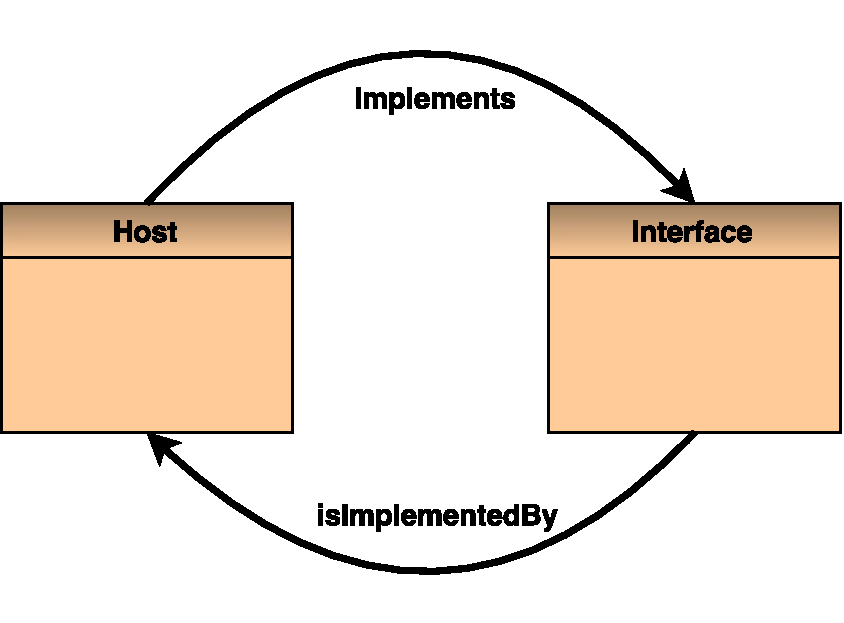
\includegraphics[scale=.55]{images/serin-discovery-classes.pdf}
	\centering
	\caption{Classes in the SERIN ontology that support the discovery process.}
	\label{fig:discoveryclass}
\end{figure}

SERIN ontology defines two classes: \textit{Host} and \textit{Interface} (Figure \ref{fig:discoveryclass}). \textit{Host} represents any machine in a network, like for example a service provider on the Web. \textit{Interface} represents any ontology that acts as a semantic interface.
Hosts are related to Interfaces through the object property \textit{implements} and its inverse property \textit{isImplementBy}. 

For example, one consider a network model with a set of hosts that attends some semantic interfaces as shown in figure \ref{fig:host-interface-example}. The class \textit{Host} has three instances \textit{MyHost}, \textit{YourHost}, and \textit{TheirHost}. The class \textit{Interface} has two instances \textit{BookInterface} and \textit{TravelInterface}. 
The property, and of course its inverse property, implements defines a relationship between Host and Interface. 
Thus, the model defines that the hosts \textit{MyHost} and \textit{YourHost} implements the interface \textit{BookInterface}, while the host \textit{TheirHost} implements the interface \textit{TravelInterface}.

\begin{figure}[!htb]
	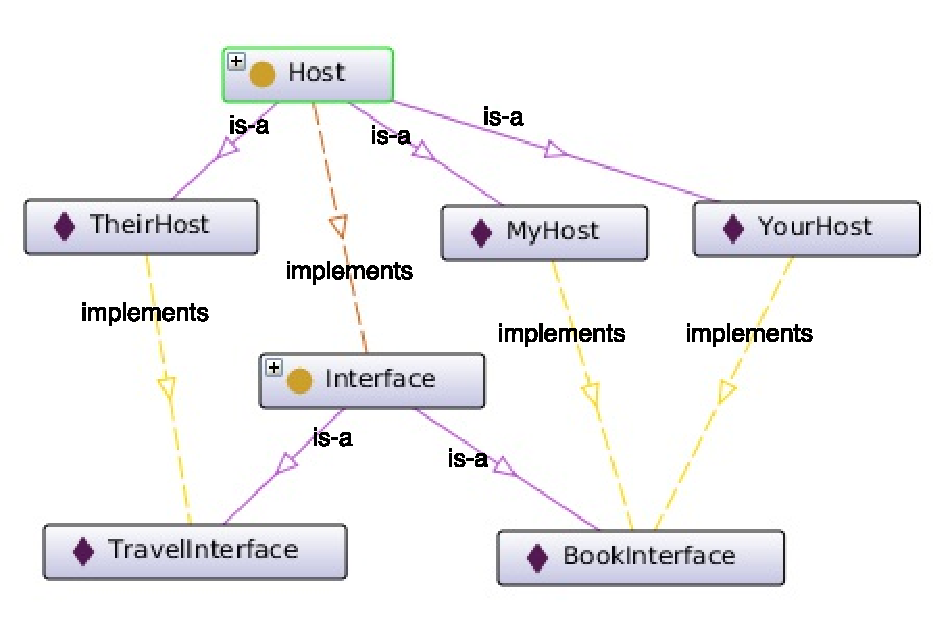
\includegraphics[scale=.45]{images/host-interface-example.pdf}
	\centering
	\caption{SERIN model for the relationship among hosts and semantic interfaces.}
	\label{fig:host-interface-example}
\end{figure}

SERIN annotations, classes, and properties present a minimal set of concepts necessary for the service discovery process.

\subsection{The Address convention}
\label{sec:addressconvention}
Besides standardize the semantics, SERIN contributes to standardize the web services URLs. 
Each URL is divided into two parts. 
The first part identifies the host. 
The second part semantically identifies the resource. 
The basic address convention format is:

\begin{lstlisting}[frame=single, basicstyle=\small\ttfamily]
http://{host}/{interface}/{class}/{resource}
\end{lstlisting}

where:

\begin{itemize}
	\item \texttt{\{host\}} - IP or DNS host address.
	\item \texttt{\{interface\}} - ontology URI that represents the semantic interface.
	\item \texttt{\{class\}} - ontology class identifier.
	\item \texttt{\{resource\}} - resource identifier.
\end{itemize}

The first part of the address is composed by the \{host\} element. 
The second part of the address is composed by the elements \{interface\}, \{class\}, and \{resource\}. These elements identifies a resource in the host defined by the element \{host\}.
The element \{resource\} is optional and it is used to request an individual resource.
When the element \{resource\} is not indicated, the element \{class\} is used to request a collection of resources from the class indicated by \{class\}.

Using this address convention, it is possible to deriver the URL of a RESTful web service from the ontology URI concatenated to the host address.  

\begin{figure}[!htb]
	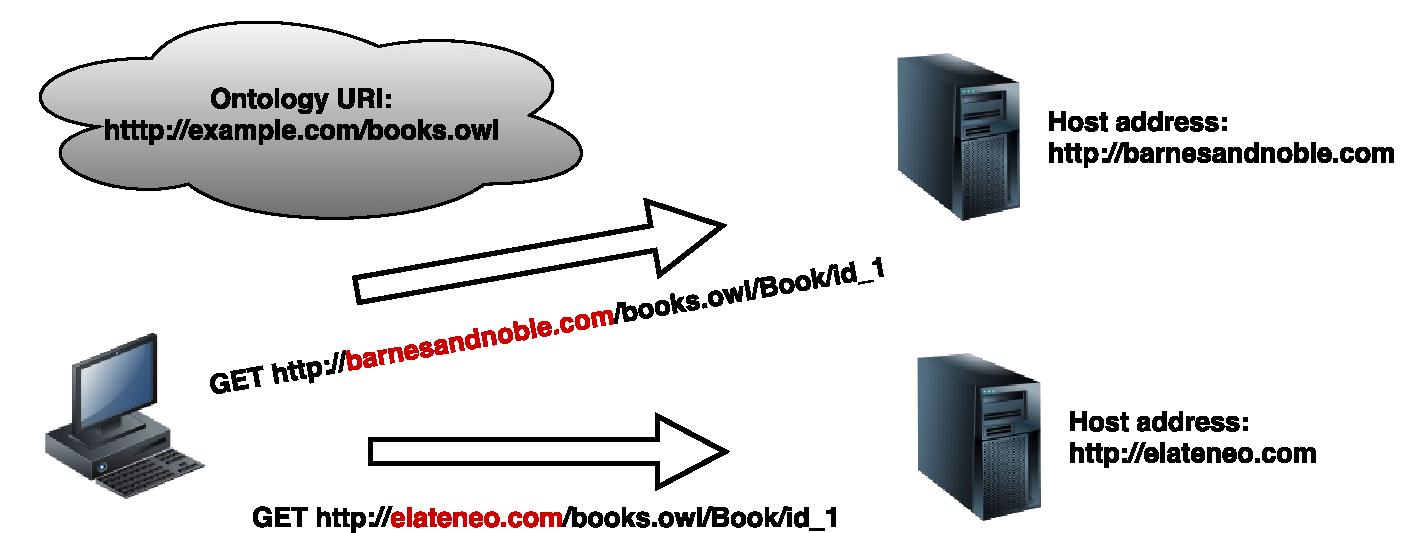
\includegraphics[scale=.5]{images/bookstore-address-convention.pdf}
	\centering
	\caption{Example of SERIN address convention in a request for the resources of a class \textit{Book}.}
	\label{fig:bookstoreadrress}
\end{figure}

In the bookstore example (Figure \ref{fig:bookstoreadrress}), a client sends two requests to obtain data about books in two hosts. Supposing that the client intends to obtain data about a book whose identification is id\_1 in the first host, the address convention composition is

\begin{lstlisting}
{host} = barnesandnoble.com
{interface} = books.owl
{class} = Book
{resource} = id_1

\end{lstlisting}

The request URL has the same pattern. The first part, colored in red in the figure, indicates the host address which is http://barnesandnoble.com for one host and http://elateneo.com for the second host. This is the variant part of the URL pattern. The second part of the request URL, which is /books.owl/Book/id\_1, is the same for all requests in the example. The second part indicates a resource from the class Book that has the identification id\_1.

%TODO (xxx) ve se da tempo: acha interessante colocar mais um exemplo tratando de internet das coisas.

Although it is particularly simple, the address convention introduces benefits to the discovery of semantic web services and to the reuse of web services and resources published on the web. 
One advantage of the address convention is that it provides a standard address to a web service that attends an interface even if the host is unknown. 
A crawler can execute an inspection to the standard web service address that follows a semantic interface. 

\subsubsection{Additional elements}
\label{sec:addressaddtional}
It is possible to add some parameters to the basic address convention in order to reduce the result set. 

The main characteristic about the parameters in SERIN address convention is that these parameters are always associated to an object property or a datatype property from a semantic interface. 
An web service that returns resources from a class can only receive as parameters the properties that are related to that class.  
This way, the semantic interface defines a schema for the parameters in a web service call.    

This is an important difference between SERIN specification and other similar approaches. 
In these approaches, the parameters usually are syntactic pairs in the form \textit{parameter=value} where the parameter is not necessarily associated to a concept in an ontology.  

\subsubsection{Filtering}
\label{sec:filtering}
Each property related to a class may work as a filter condition. The address convention to add filtering is 
% The following parameters provide features to filter resources and to select the objects that the services shall return.

\begin{lstlisting}[frame=single, basicstyle=\small\ttfamily]
http://{host}/{interface}/{class}?{property}={value}
\end{lstlisting}

where:

\begin{itemize}
	\item \texttt{\{property\}} - A property in the \textbf{{interface}} ontology that is related with the \textbf{{class}}. It can be either a datatype property or an object property.
	\item \texttt{\{value\}} - The value attribute for this property. A URI can assume the value in case of an object property.
\end{itemize}

The address convention allows the use of the ampersand (\&) operator to add optional property=value pairs.

Considering the example in the Figure \ref{fig:bookstoreadrress}, it is possible to refine the search using these parameters.

Using the basic SERIN address convention, the request 

\begin{lstlisting}
GET /example.com/books.owl/Book
\end{lstlisting}

returns the list of all books in the host database, which is a too wide response. On the other side, the request 

\begin{lstlisting}
GET /example.com/books.owl/Book/id_1
\end{lstlisting}

returns data about only one specific book, which is a very restrictive query.

The parameters enables the web services to provide responses with a set of resources that are in the middle of these two previous requests.

The following request ask for all books whose title is Moby Dick.

\begin{lstlisting}[breaklines=true]
GET /example.com/books.owl/Book?title="Moby Dick"
\end{lstlisting}

The ampersand (\&) can restrict even more the result set as in 

\begin{lstlisting}[breaklines=true]
GET /example.com/books.owl/Book?title="Moby Dick"&editor="Penguin"
\end{lstlisting}

which returns all books with title Moby Dick and that the editor is Penguin.

\subsubsection{Result set restrictors}
\label{sec:otherparam}
Other special operators defined in the SERIN address convention specification are:

\begin{itemize}
	\item \texttt{properties} - The requester may inform a list of properties to be returned. The result set will present only the properties in this list.
	\item \texttt{query} - The requester may build a more complex query using logical and boolean operators. Note that the objects in the query are the ones contained in the semantic interface.
	\item \texttt{size} - It limits the number of returned occurrences.
	\item \texttt{page} - It enables pagination of the returned occurences.
\end{itemize}

Adding these operators, the address convention syntax is

\begin{lstlisting}[frame=single, basicstyle=\small\ttfamily, breaklines=true]
http://{host}/{interface}/{class}?{property}={value}&properties=({property 1}/.../{property N})&size=x&page=n
\end{lstlisting}

In the bookstore example, if the client needs a response with data about a book with only the properties title, isbn and author name, the client sends the request:  

\begin{lstlisting}[breaklines=true]
http:///example.com/books.owl/Book?properties=(title/isbn/author(name))
\end{lstlisting}

The result set of books can be reduced to a limited number of 200 resources in the following request. We intend to improve the response time distributing the resources in pages of 10 elements. The request returns the first page.

\begin{lstlisting}[breaklines=true]
http:///example.com/books.owl/Book?size=200&page=1
\end{lstlisting}

These parameters can all be combined in a more complete request:

\begin{lstlisting}[breaklines=true]
http:///example.com/books.owl/Book?title=Moby Dick&properties=(title/isbn/author(name))&size=200&page=1
\end{lstlisting}

\section{Comparison between SERIN and previous approaches}
\label{sec:comparison}

\subsection{Comparison between SERIN and ReLL}
\label{sec:rell-implement}

\subsubsection{Twitter semantic interface implementation}
\label{sec:twitter-implement}

\subsubsection{Flickr semantic interface implementation}
\label{sec:flickr-implement}

\subsubsection{School semantic interface implementation}
\label{sec:school-implement}

\subsubsection{SERIN alternative to the concept usermap}
\label{sec:user-map}

\subsection{Comparison between SERIN and hRESTs/MicroWSMO}
\label{sec:hrests-implement}

\subsubsection{Analysis of web service descriptions}
\label{sec:}

\subsubsection{SERIN similar implementation}
\label{sec:hrestcomparison}

\subsection{Comparison between SERIN and RESTdesc}
\label{sec:restdesc-implement}

\subsubsection{RESTdesc example using SERIN}
\label{sec:restdesccomparison}

\section{Conclusion}
\label{sec:conclusion}


\bibliographystyle{apalike}
\bibliography{Mendeley}

\end{document}
